% Options for packages loaded elsewhere
\PassOptionsToPackage{unicode}{hyperref}
\PassOptionsToPackage{hyphens}{url}
%
\documentclass[
  11pt,
  ignorenonframetext,
]{beamer}
\usepackage{pgfpages}
\setbeamertemplate{caption}[numbered]
\setbeamertemplate{caption label separator}{: }
\setbeamercolor{caption name}{fg=normal text.fg}
\beamertemplatenavigationsymbolsempty
% Prevent slide breaks in the middle of a paragraph
\widowpenalties 1 10000
\raggedbottom
\setbeamertemplate{part page}{
  \centering
  \begin{beamercolorbox}[sep=16pt,center]{part title}
    \usebeamerfont{part title}\insertpart\par
  \end{beamercolorbox}
}
\setbeamertemplate{section page}{
  \centering
  \begin{beamercolorbox}[sep=12pt,center]{part title}
    \usebeamerfont{section title}\insertsection\par
  \end{beamercolorbox}
}
\setbeamertemplate{subsection page}{
  \centering
  \begin{beamercolorbox}[sep=8pt,center]{part title}
    \usebeamerfont{subsection title}\insertsubsection\par
  \end{beamercolorbox}
}
\AtBeginPart{
  \frame{\partpage}
}
\AtBeginSection{
  \ifbibliography
  \else
    \frame{\sectionpage}
  \fi
}
\AtBeginSubsection{
  \frame{\subsectionpage}
}

\usepackage{amsmath,amssymb}
\usepackage{iftex}
\ifPDFTeX
  \usepackage[T1]{fontenc}
  \usepackage[utf8]{inputenc}
  \usepackage{textcomp} % provide euro and other symbols
\else % if luatex or xetex
  \usepackage{unicode-math}
  \defaultfontfeatures{Scale=MatchLowercase}
  \defaultfontfeatures[\rmfamily]{Ligatures=TeX,Scale=1}
\fi
\usepackage{lmodern}
\usetheme[]{AnnArbor}
\usecolortheme{seahorse}
\ifPDFTeX\else  
    % xetex/luatex font selection
\fi
% Use upquote if available, for straight quotes in verbatim environments
\IfFileExists{upquote.sty}{\usepackage{upquote}}{}
\IfFileExists{microtype.sty}{% use microtype if available
  \usepackage[]{microtype}
  \UseMicrotypeSet[protrusion]{basicmath} % disable protrusion for tt fonts
}{}
\makeatletter
\@ifundefined{KOMAClassName}{% if non-KOMA class
  \IfFileExists{parskip.sty}{%
    \usepackage{parskip}
  }{% else
    \setlength{\parindent}{0pt}
    \setlength{\parskip}{6pt plus 2pt minus 1pt}}
}{% if KOMA class
  \KOMAoptions{parskip=half}}
\makeatother
\usepackage{xcolor}
\newif\ifbibliography
\setlength{\emergencystretch}{3em} % prevent overfull lines
\setcounter{secnumdepth}{5}

\usepackage{color}
\usepackage{fancyvrb}
\newcommand{\VerbBar}{|}
\newcommand{\VERB}{\Verb[commandchars=\\\{\}]}
\DefineVerbatimEnvironment{Highlighting}{Verbatim}{commandchars=\\\{\}}
% Add ',fontsize=\small' for more characters per line
\usepackage{framed}
\definecolor{shadecolor}{RGB}{241,243,245}
\newenvironment{Shaded}{\begin{snugshade}}{\end{snugshade}}
\newcommand{\AlertTok}[1]{\textcolor[rgb]{0.68,0.00,0.00}{#1}}
\newcommand{\AnnotationTok}[1]{\textcolor[rgb]{0.37,0.37,0.37}{#1}}
\newcommand{\AttributeTok}[1]{\textcolor[rgb]{0.40,0.45,0.13}{#1}}
\newcommand{\BaseNTok}[1]{\textcolor[rgb]{0.68,0.00,0.00}{#1}}
\newcommand{\BuiltInTok}[1]{\textcolor[rgb]{0.00,0.23,0.31}{#1}}
\newcommand{\CharTok}[1]{\textcolor[rgb]{0.13,0.47,0.30}{#1}}
\newcommand{\CommentTok}[1]{\textcolor[rgb]{0.37,0.37,0.37}{#1}}
\newcommand{\CommentVarTok}[1]{\textcolor[rgb]{0.37,0.37,0.37}{\textit{#1}}}
\newcommand{\ConstantTok}[1]{\textcolor[rgb]{0.56,0.35,0.01}{#1}}
\newcommand{\ControlFlowTok}[1]{\textcolor[rgb]{0.00,0.23,0.31}{#1}}
\newcommand{\DataTypeTok}[1]{\textcolor[rgb]{0.68,0.00,0.00}{#1}}
\newcommand{\DecValTok}[1]{\textcolor[rgb]{0.68,0.00,0.00}{#1}}
\newcommand{\DocumentationTok}[1]{\textcolor[rgb]{0.37,0.37,0.37}{\textit{#1}}}
\newcommand{\ErrorTok}[1]{\textcolor[rgb]{0.68,0.00,0.00}{#1}}
\newcommand{\ExtensionTok}[1]{\textcolor[rgb]{0.00,0.23,0.31}{#1}}
\newcommand{\FloatTok}[1]{\textcolor[rgb]{0.68,0.00,0.00}{#1}}
\newcommand{\FunctionTok}[1]{\textcolor[rgb]{0.28,0.35,0.67}{#1}}
\newcommand{\ImportTok}[1]{\textcolor[rgb]{0.00,0.46,0.62}{#1}}
\newcommand{\InformationTok}[1]{\textcolor[rgb]{0.37,0.37,0.37}{#1}}
\newcommand{\KeywordTok}[1]{\textcolor[rgb]{0.00,0.23,0.31}{#1}}
\newcommand{\NormalTok}[1]{\textcolor[rgb]{0.00,0.23,0.31}{#1}}
\newcommand{\OperatorTok}[1]{\textcolor[rgb]{0.37,0.37,0.37}{#1}}
\newcommand{\OtherTok}[1]{\textcolor[rgb]{0.00,0.23,0.31}{#1}}
\newcommand{\PreprocessorTok}[1]{\textcolor[rgb]{0.68,0.00,0.00}{#1}}
\newcommand{\RegionMarkerTok}[1]{\textcolor[rgb]{0.00,0.23,0.31}{#1}}
\newcommand{\SpecialCharTok}[1]{\textcolor[rgb]{0.37,0.37,0.37}{#1}}
\newcommand{\SpecialStringTok}[1]{\textcolor[rgb]{0.13,0.47,0.30}{#1}}
\newcommand{\StringTok}[1]{\textcolor[rgb]{0.13,0.47,0.30}{#1}}
\newcommand{\VariableTok}[1]{\textcolor[rgb]{0.07,0.07,0.07}{#1}}
\newcommand{\VerbatimStringTok}[1]{\textcolor[rgb]{0.13,0.47,0.30}{#1}}
\newcommand{\WarningTok}[1]{\textcolor[rgb]{0.37,0.37,0.37}{\textit{#1}}}

\providecommand{\tightlist}{%
  \setlength{\itemsep}{0pt}\setlength{\parskip}{0pt}}\usepackage{longtable,booktabs,array}
\usepackage{calc} % for calculating minipage widths
\usepackage{caption}
% Make caption package work with longtable
\makeatletter
\def\fnum@table{\tablename~\thetable}
\makeatother
\usepackage{graphicx}
\makeatletter
\def\maxwidth{\ifdim\Gin@nat@width>\linewidth\linewidth\else\Gin@nat@width\fi}
\def\maxheight{\ifdim\Gin@nat@height>\textheight\textheight\else\Gin@nat@height\fi}
\makeatother
% Scale images if necessary, so that they will not overflow the page
% margins by default, and it is still possible to overwrite the defaults
% using explicit options in \includegraphics[width, height, ...]{}
\setkeys{Gin}{width=\maxwidth,height=\maxheight,keepaspectratio}
% Set default figure placement to htbp
\makeatletter
\def\fps@figure{htbp}
\makeatother

\usepackage{booktabs}
\usepackage{longtable}
\usepackage{array}
\usepackage{multirow}
\usepackage{wrapfig}
\usepackage{float}
\usepackage{colortbl}
\usepackage{pdflscape}
\usepackage{tabu}
\usepackage{threeparttable}
\usepackage{threeparttablex}
\usepackage[normalem]{ulem}
\usepackage{makecell}
\usepackage{xcolor}
\usepackage{amsmath, amssymb, bbm, amstext, array, listings, mathtools, caption, color, graphics, ulem, caption, changepage, atbegshi, soul}
\newcommand\E{\mathbb{E}}
\newcommand\V{\mathbb{V}}
\hypersetup{colorlinks=true,linkcolor=red}
\usepackage{ulem}
\pdfstringdefDisableCommands{\let\sout\relax}
\makeatletter
\makeatother
\makeatletter
\makeatother
\makeatletter
\@ifpackageloaded{caption}{}{\usepackage{caption}}
\AtBeginDocument{%
\ifdefined\contentsname
  \renewcommand*\contentsname{Table of contents}
\else
  \newcommand\contentsname{Table of contents}
\fi
\ifdefined\listfigurename
  \renewcommand*\listfigurename{List of Figures}
\else
  \newcommand\listfigurename{List of Figures}
\fi
\ifdefined\listtablename
  \renewcommand*\listtablename{List of Tables}
\else
  \newcommand\listtablename{List of Tables}
\fi
\ifdefined\figurename
  \renewcommand*\figurename{Figure}
\else
  \newcommand\figurename{Figure}
\fi
\ifdefined\tablename
  \renewcommand*\tablename{Table}
\else
  \newcommand\tablename{Table}
\fi
}
\@ifpackageloaded{float}{}{\usepackage{float}}
\floatstyle{ruled}
\@ifundefined{c@chapter}{\newfloat{codelisting}{h}{lop}}{\newfloat{codelisting}{h}{lop}[chapter]}
\floatname{codelisting}{Listing}
\newcommand*\listoflistings{\listof{codelisting}{List of Listings}}
\makeatother
\makeatletter
\@ifpackageloaded{caption}{}{\usepackage{caption}}
\@ifpackageloaded{subcaption}{}{\usepackage{subcaption}}
\makeatother
\makeatletter
\@ifpackageloaded{tcolorbox}{}{\usepackage[skins,breakable]{tcolorbox}}
\makeatother
\makeatletter
\@ifundefined{shadecolor}{\definecolor{shadecolor}{rgb}{.97, .97, .97}}
\makeatother
\makeatletter
\makeatother
\makeatletter
\makeatother
\ifLuaTeX
  \usepackage{selnolig}  % disable illegal ligatures
\fi
\IfFileExists{bookmark.sty}{\usepackage{bookmark}}{\usepackage{hyperref}}
\IfFileExists{xurl.sty}{\usepackage{xurl}}{} % add URL line breaks if available
\urlstyle{same} % disable monospaced font for URLs
\hypersetup{
  pdftitle={Lectures on causal inference and experimental methods},
  pdfauthor={Macartan Humphreys},
  hidelinks,
  pdfcreator={LaTeX via pandoc}}

\title{Lectures on causal inference and experimental methods}
\author{Macartan Humphreys}
\date{}

\begin{document}
\frame{\titlepage}
\ifdefined\Shaded\renewenvironment{Shaded}{\begin{tcolorbox}[interior hidden, frame hidden, borderline west={3pt}{0pt}{shadecolor}, sharp corners, boxrule=0pt, enhanced, breakable]}{\end{tcolorbox}}\fi

\hypertarget{inquiries}{%
\section{\texorpdfstring{Inquiries
\label{estimands}}{Inquiries }}\label{inquiries}}

\hypertarget{estimands-and-inquiries}{%
\subsection{Estimands and inquiries}\label{estimands-and-inquiries}}

\begin{frame}{Estimands and inquiries}
\begin{itemize}
\tightlist
\item
  Your inquiry is your question and the estimand is the true (generally
  unknown) answer to the inquiry
\item
  The estimand is the thing you want to estimate
\item
  If you are estimating something you should be able to say what your
  estimand is
\item
  You are responsible for your estimand. Your estimator will not tell
  you what your estimand is
\item
  Just because you can calculate something does not mean that you have
  an estimand
\item
  You can test a hypothesis without having an estimand
\end{itemize}

Read:
\href{https://macartan.github.io/integrated_inferences/HJC4.html}{II ch
4},
\href{https://book.declaredesign.org/declaration-diagnosis-redesign/defining-inquiry.html}{DD,
ch 7}
\end{frame}

\begin{frame}[fragile]{Estimands: ATE, ATT, ATC, S-, P-, C-, ITT, LATE}
\protect\hypertarget{estimands-ate-att-atc-s--p--c--itt-late}{}
Say that units are randomly assigned to treatment in different strata
(maybe just one); with fixed, though possibly different, shares assigned
in each stratum. Then the key estimands and estimators are:

\begin{longtable}[]{@{}
  >{\raggedright\arraybackslash}p{(\columnwidth - 2\tabcolsep) * \real{0.4356}}
  >{\raggedright\arraybackslash}p{(\columnwidth - 2\tabcolsep) * \real{0.5644}}@{}}
\toprule\noalign{}
\begin{minipage}[b]{\linewidth}\raggedright
Estimand
\end{minipage} & \begin{minipage}[b]{\linewidth}\raggedright
Estimator
\end{minipage} \\
\midrule\noalign{}
\endhead
\(\tau_{ATE} \equiv \mathbb{E}[\tau_i]\) &
\(\widehat{\tau}_{ATE} = \sum\nolimits_{x} \frac{w_x}{\sum\nolimits_{j}w_{j}}\widehat{\tau}_x\) \\
\(\tau_{ATT} \equiv \mathbb{E}[\tau_i | Z_i = 1]\) &
\(\widehat{\tau}_{ATT} = \sum\nolimits_{x} \frac{p_xw_x}{\sum\nolimits_{j}p_jw_j}\widehat{\tau}_x\) \\
\(\tau_{ATC} \equiv \mathbb{E}[\tau_i | Z_i = 0]\) &
\(\widehat{\tau}_{ATC} = \sum\nolimits_{x} \frac{(1-p_x)w_x}{\sum\nolimits_{j}(1-p_j)w_j}\widehat{\tau}_x\) \\
\bottomrule\noalign{}
\end{longtable}

where \(x\) indexes strata, \(p_x\) is the share of units in each
stratum that is treated, and \(w_x\) is the size of a stratum.

Here:

\begin{verbatim}
* ATE is Average Treatment Effect (all units)
* ATT is Average Treatment Effect on the Treated
* ATC is Average Treatment Effect on the Controls
\end{verbatim}
\end{frame}

\begin{frame}{Estimands: ATE, ATT, ATC, S-, P-, C-, ITT, LATE}
\protect\hypertarget{estimands-ate-att-atc-s--p--c--itt-late-1}{}
In addition, each of these can be targets of interest:

\begin{itemize}
\tightlist
\item
  for the \textbf{population}, in which case we refer to PATE, PATT,
  PATC and \(\widehat{PATE}, \widehat{PATT}, \widehat{PATC}\)
\item
  for a \textbf{sample}, in which case we refer to SATE, SATT, SATC, and
  \(\widehat{SATE}, \widehat{SATT}, \widehat{SATC}\)
\end{itemize}

And for different subgroups,

\begin{itemize}
\tightlist
\item
  given some value on a covariate, in which case we refer to CATE
  (conditional average treatment effect)
\item
  for unobservable subgroups, we estimate LATE (Local Average Treatment
  Effect (see below).
\end{itemize}

With non-compliance we might estimate ITT ---the ``intention to treat''
effect
\end{frame}

\hypertarget{mediation-estimands-and-complex-counterfactuals}{%
\subsection{Mediation estimands and complex
counterfactuals}\label{mediation-estimands-and-complex-counterfactuals}}

\hypertarget{causes-of-effects-and-effects-of-causes}{%
\subsection{Causes of effects and effects of
causes}\label{causes-of-effects-and-effects-of-causes}}

\hypertarget{actual-causation}{%
\subsection{Actual causation}\label{actual-causation}}

\hypertarget{pearls-ladder}{%
\subsection{Pearl's ladder}\label{pearls-ladder}}

\hypertarget{inquiries-as-statements-about-principal-strata}{%
\subsection{Inquiries as statements about principal
strata}\label{inquiries-as-statements-about-principal-strata}}

\hypertarget{identification}{%
\subsection{Identification}\label{identification}}

\begin{frame}{Identification}
\emph{What it is. When you have it. What it's worth.}
\end{frame}

\begin{frame}{Identification}
\protect\hypertarget{identification-1}{}
\end{frame}

\begin{frame}{Identification : Goal}
\protect\hypertarget{identification-goal}{}
Our goal in causal inference is to estimate quantities such as:

\[\Pr(Y|\hat{x})\]

where \(\hat{x}\) is interpreted as \(X\) set to \(x\) by ``external''
control. Equivalently: \(do(X=x)\) or sometimes \(X \leftarrow x\).

For example for a binary \(X, Y\) the causal effect of \(X\) on the
probability that \(Y=1\) is:

\[\Pr(Y=1|\hat{x}=1) - \Pr(Y=1|\hat{x}=0)\]

In general though \textbf{this is not the same as}:

\[\Pr(Y=1|x=1) - \Pr(Y=1|x=0)\]

It's the difference between seeing and doing.
\end{frame}

\begin{frame}[fragile]{When to condition? What to condition on?}
\protect\hypertarget{when-to-condition-what-to-condition-on}{}
The key idea is that you want to find a set of variables such that when
you condition on these you get what you would get if you used a
\texttt{do} operation. For this you want to make sure that there are no
``backdoor'' paths between \(X\) and \(Y\).

Intuition:

\begin{itemize}
\tightlist
\item
  You could imagine creating a ``mutilated'' graph by removing all the
  arrows leading \emph{out} of \emph{X}
\item
  Then select a set of variables, \(Z\), such that \(X\) and \(Y\) are
  d-separated by \(Z\) on the the mutilated graph
\item
  When you condition on these you are making sure that any covariation
  between \(X\) and \(Y\) is covariation that is due to the effects of
  \(X\)
\end{itemize}
\end{frame}

\begin{frame}{Illustration}
\protect\hypertarget{illustration}{}
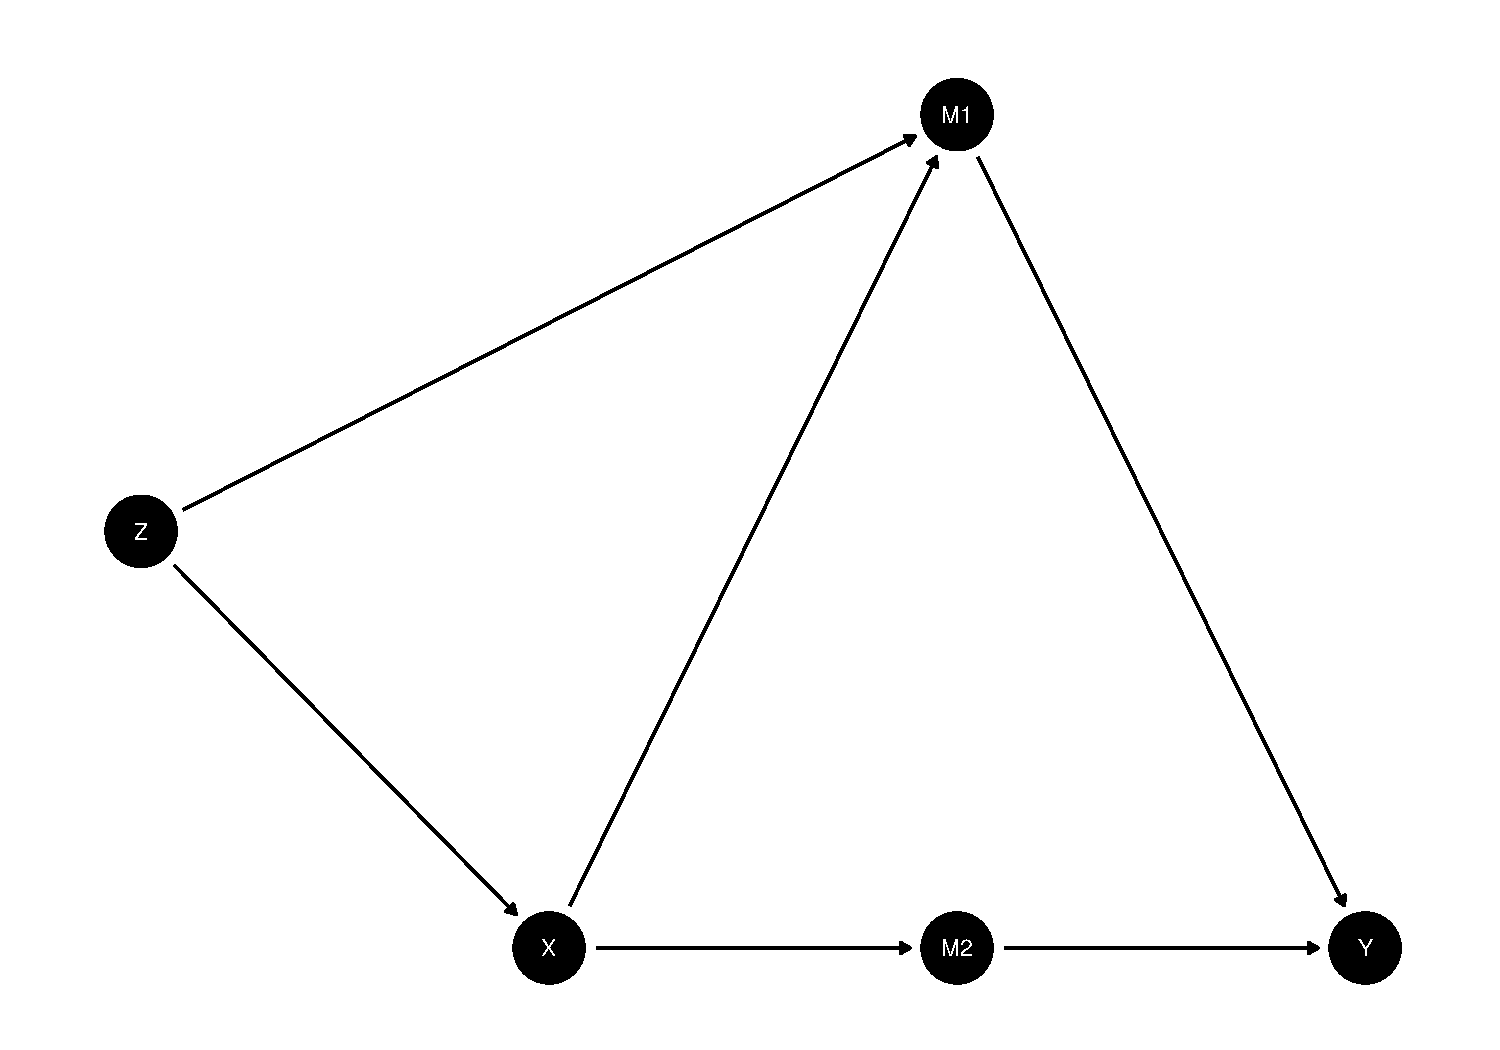
\includegraphics{2.2_estimands_files/figure-beamer/unnamed-chunk-2-1.pdf}
\end{frame}

\begin{frame}{Illustration: Remove paths out}
\protect\hypertarget{illustration-remove-paths-out}{}
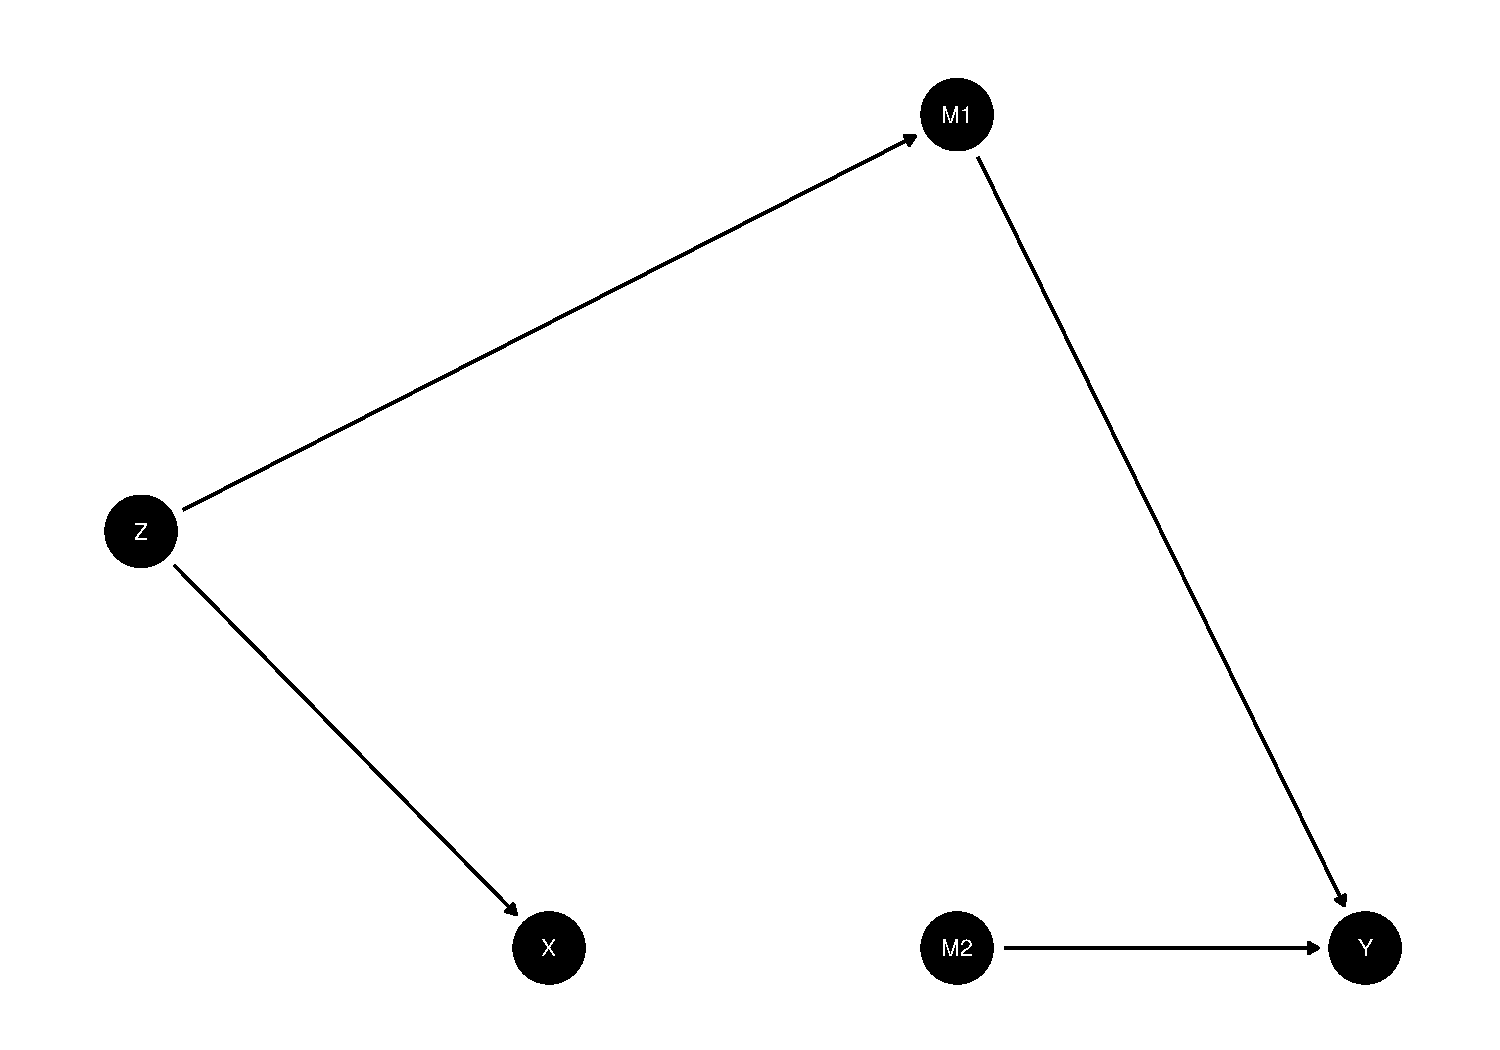
\includegraphics{2.2_estimands_files/figure-beamer/unnamed-chunk-3-1.pdf}
\end{frame}

\begin{frame}{Illustration: Block backdoor path}
\protect\hypertarget{illustration-block-backdoor-path}{}
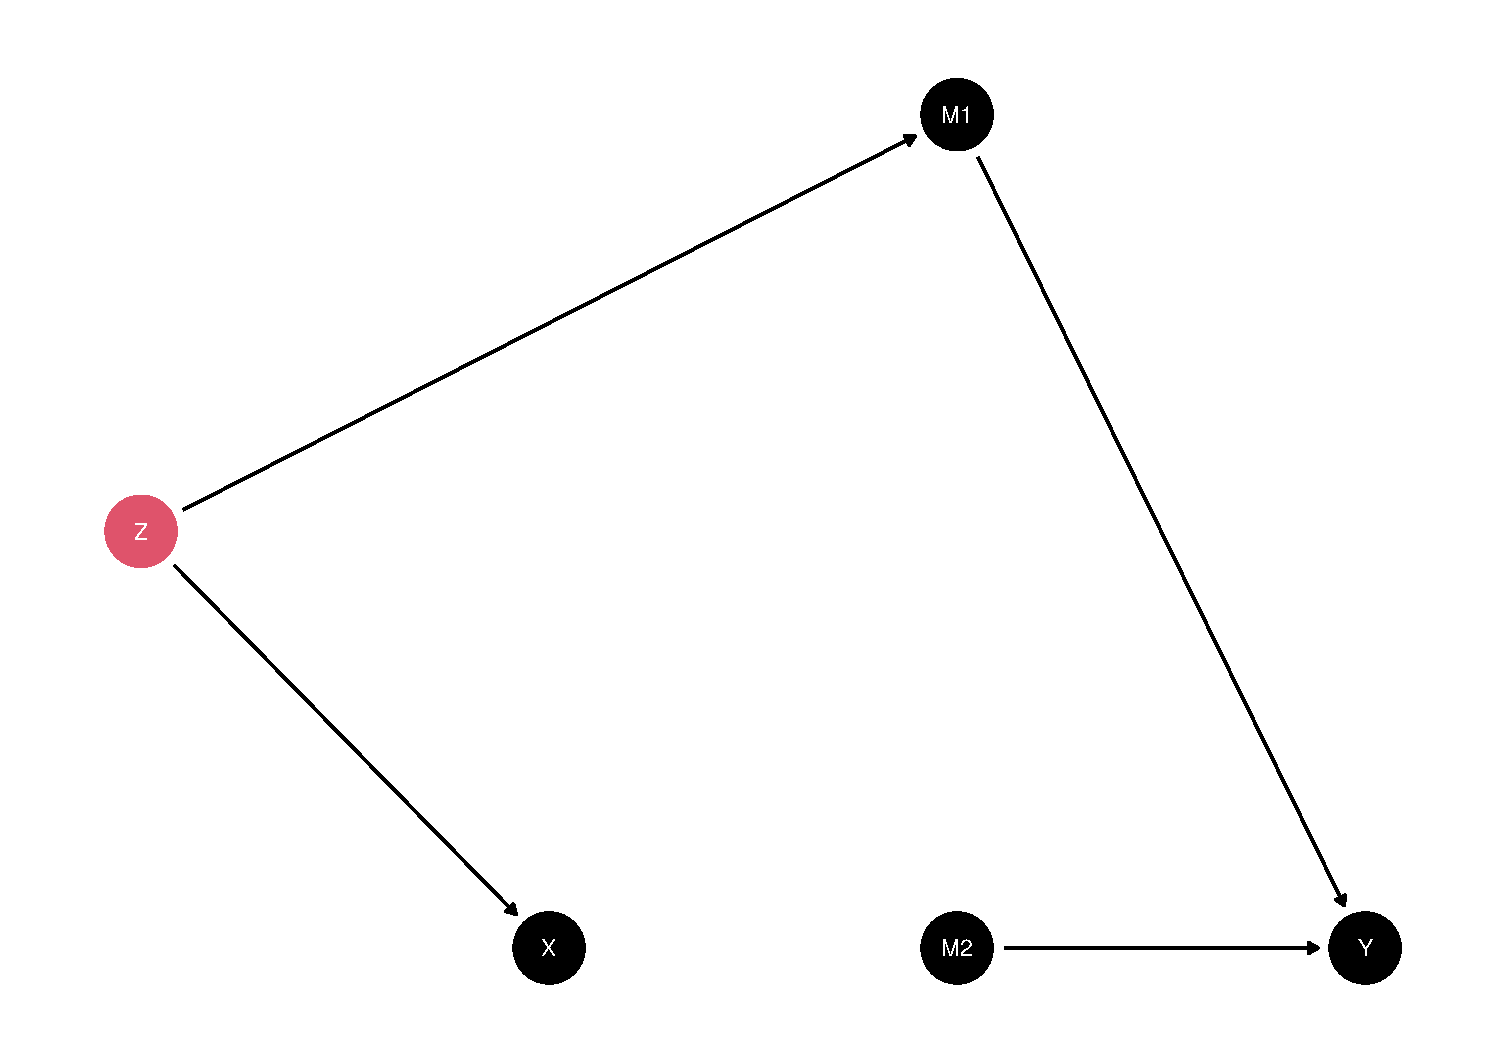
\includegraphics{2.2_estimands_files/figure-beamer/unnamed-chunk-4-1.pdf}
\end{frame}

\begin{frame}{Illustration: Why not like this?}
\protect\hypertarget{illustration-why-not-like-this}{}
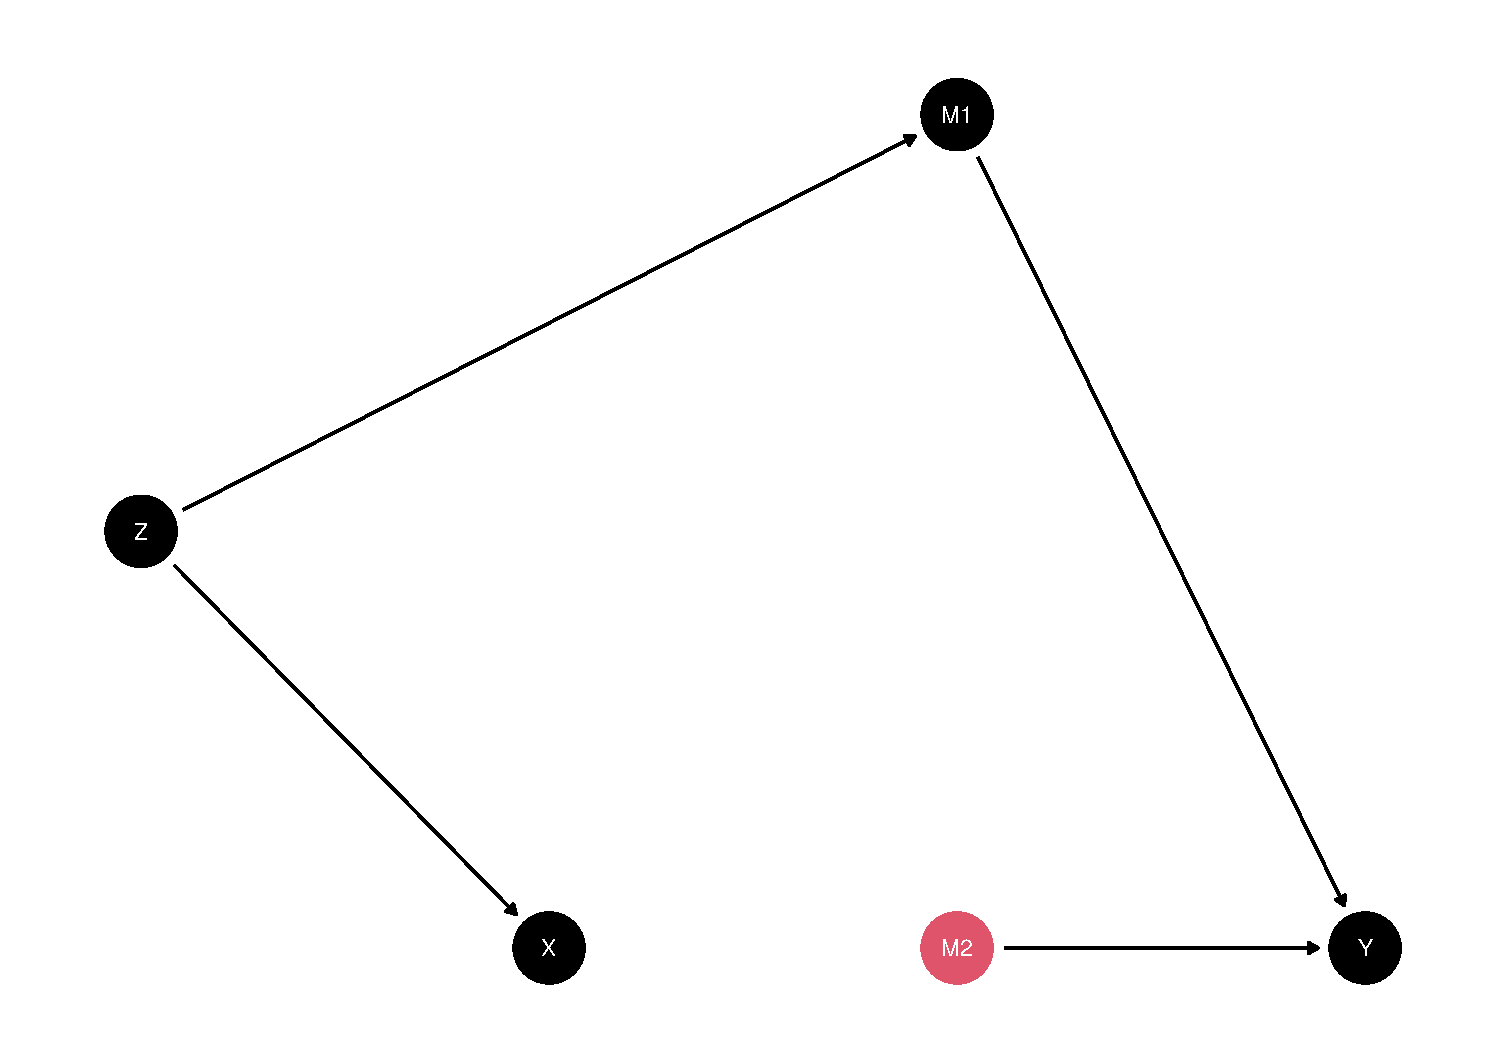
\includegraphics{2.2_estimands_files/figure-beamer/unnamed-chunk-5-1.pdf}
\end{frame}

\begin{frame}{Identification}
\protect\hypertarget{identification-2}{}
\begin{itemize}
\tightlist
\item
  Three results (``Graphical Identification Criteria'')

  \begin{itemize}
  \tightlist
  \item
    Backdoor criterion
  \item
    Adjustment criterion
  \item
    Frontdoor criterion
  \end{itemize}
\item
  There are more
\end{itemize}
\end{frame}

\begin{frame}{Backdoor Criterion: (Pearl 1995)}
\protect\hypertarget{backdoor-criterion-pearl-1995}{}
The \textbf{backdoor criterion} is satisfied by \(Z\) (relative to
\(X\), \(Y\)) if:

\begin{enumerate}
\tightlist
\item
  No node in \(Z\) is a descendant of \(X\)
\item
  \(Z\) blocks every \textbf{backdoor} path from \(X\) to \(Y\)
  (i.e.~every path that contains an arrow into \(X\))
\end{enumerate}

In that case you can identify the effect of \(X\) on \(Y\) by
conditioning on \(Z\):

\[P(Y=y | \hat{x}) = \sum_z P(Y=y| X = x, Z=z)P(z)\] (This is eqn 3.19
in Pearl (2000))
\end{frame}

\begin{frame}{Backdoor Criterion: (Pearl 1995)}
\protect\hypertarget{backdoor-criterion-pearl-1995-1}{}
\[P(Y=y | \hat{x}) = \sum_z P(Y=y| X = x, Z=z)P(z)\]

\begin{itemize}
\tightlist
\item
  Note notion of a linear control of anything like that; idea really is
  like blocking: think lots of discrete data and no missing patterns
\item
  Note this is a formula for a (possibly counterfactual) \emph{level}; a
  counterfactual difference would be given in the obvious way by:
\end{itemize}

\[P(Y=y | \hat{x}) - P(Y=y | \hat{x}') = \sum_z P(Y=y| X = x, Z=z)P(z) - \sum_z P(Y=y| X = x', Z=z)P(z)\]
\end{frame}

\begin{frame}{Backdoor Proof}
\protect\hypertarget{backdoor-proof}{}
Following Pearl (2009), Chapter 11. Let \(T\) denote the set of parents
of \(X\): \(T := pa(X)\), with (possibly vector valued) realizations
\(t\).

If the backdoor criterion is satisfied, we have:

\begin{enumerate}
\tightlist
\item
  \(Y\) is independent of \(T\), given \(X\) and observed data, \(Z\)
  (since \(Z\) blocks backdoor paths)
\item
  \(X\) is independent of \(Z\) given \(T\). (Since \(Z\) includes only
  nondescendents)
\end{enumerate}

\begin{itemize}
\tightlist
\item
  From the DAG we have:
  \[p(y|\hat{x}) = \sum_{t\in T} p(t)p(y|\hat{x}, t)\]
\end{itemize}
\end{frame}

\begin{frame}{Backdoor Proof}
\protect\hypertarget{backdoor-proof-1}{}
\begin{itemize}
\item
  But we do not observe \(T\), rather we observe \(Z\). OK, but we can
  write:
  \[p(y|\hat{x}) = \sum_{t\in T} p(t) \sum_z p(y|\hat{x}, t, z)p(z|\hat{x}, pa(X))\]
\item
  Then using the two conditions above:

  \begin{enumerate}
  \tightlist
  \item
    replace \(p(y|\hat{x}, pa(X), z)\) with \(p(y, \hat{x}, z)\)
  \item
    replace \(p(z|\hat{x}, pa(X))\) with \(p(z|\hat{x})\)
  \end{enumerate}

  This gives:
  \[p(y|\hat{x}) = \sum_{pa(X)} p(pa(X)) \sum_z p(y|\hat{x}, z)p(z|pa(X)) \]
\end{itemize}
\end{frame}

\begin{frame}{Now Clean up:}
\protect\hypertarget{now-clean-up}{}
\[p(y|\hat{x}) = \sum_{pa(X)} p(pa(X)) \sum_z p(y|\hat{x}, z)p(z|pa(X))\]
\[\leftrightarrow\]
\[p(y|\hat{x}) =  \sum_z p(y|\hat{x}, z)\sum_{pa(X)} p(pa(X))p(z|pa(X)) = \sum_z p(y|\hat{x})p(z)\]
\end{frame}

\begin{frame}{Adjustment criterion}
\protect\hypertarget{adjustment-criterion}{}
See @shpitser2012validity

The adjustment criterion is satisfied by \(Z\) (relative to \(X\),
\(Y\)) if:

\begin{enumerate}
\tightlist
\item
  no element of \(Z\) is a descendant (in the mutilated
  graph\footnote<.->{remove arrows pointing into \(X\)}) of any variable
  \(W\not\in X\) which lies on a proper causal path from \(X\) to
  \(Y\)\footnote<.->{A \emph{proper} causal pathway nodes in \(X\) to
    nodes in \(Y\) only intersects \(X\) at the endpoint}
\item
  \(Z\) blocks all \textbf{noncausal paths} from \(X\) to \(Y\)
\end{enumerate}
\end{frame}

\begin{frame}{These are different. Simple illustration.}
\protect\hypertarget{these-are-different.-simple-illustration.}{}
Here \(Z\) satisfies the adjustment criterion but not the backdoor
criterion:

\begin{figure}

{\centering 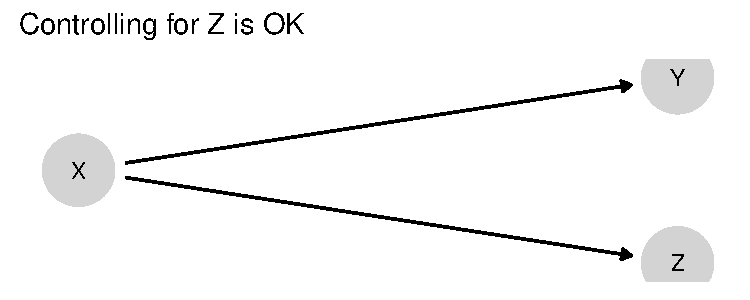
\includegraphics{2.2_estimands_files/figure-beamer/unnamed-chunk-6-1.pdf}

}

\end{figure}

\(Z\) is descendant of \(X\) but it does not a descendant of a node on a
path from \(X\) to \(Y\). No harm adjusting for \(Z\) here, but not
necessary either.
\end{frame}

\begin{frame}{Frontdoor criterion}
\protect\hypertarget{frontdoor-criterion}{}
\end{frame}

\begin{frame}[fragile]{In code: Dagitty}
\protect\hypertarget{in-code-dagitty}{}
There is a package for this

\begin{Shaded}
\begin{Highlighting}[]
\FunctionTok{library}\NormalTok{(dagitty)}
\end{Highlighting}
\end{Shaded}

Then define a dag using dagitty syntax:

\begin{Shaded}
\begin{Highlighting}[]
\NormalTok{g }\OtherTok{\textless{}{-}} \FunctionTok{dagitty}\NormalTok{(}\StringTok{"dag\{X {-}\textgreater{} M {-}\textgreater{} Y ; Z {-}\textgreater{} X ; Z {-}\textgreater{} R {-}\textgreater{} Y\}"}\NormalTok{)}
\end{Highlighting}
\end{Shaded}

There is then a simple command to check whether two sets are d-separated
by a third set:

\begin{Shaded}
\begin{Highlighting}[]
\FunctionTok{dseparated}\NormalTok{(g, }\StringTok{"X"}\NormalTok{, }\StringTok{"Y"}\NormalTok{, }\StringTok{"M"}\NormalTok{)}
\end{Highlighting}
\end{Shaded}

{[}1{]} FALSE

\begin{Shaded}
\begin{Highlighting}[]
\FunctionTok{dseparated}\NormalTok{(g, }\StringTok{"X"}\NormalTok{, }\StringTok{"Y"}\NormalTok{, }\FunctionTok{c}\NormalTok{(}\StringTok{"Z"}\NormalTok{,}\StringTok{"M"}\NormalTok{))}
\end{Highlighting}
\end{Shaded}

{[}1{]} TRUE
\end{frame}

\begin{frame}[fragile]{Dagitty: Find adjustment sets}
\protect\hypertarget{dagitty-find-adjustment-sets}{}
And a simple command to identify the adjustments needed to identify the
effect of one variable on another:

\begin{Shaded}
\begin{Highlighting}[]
\FunctionTok{adjustmentSets}\NormalTok{(g, }\AttributeTok{exposure =} \StringTok{"X"}\NormalTok{, }\AttributeTok{outcome =} \StringTok{"Y"}\NormalTok{)}
\end{Highlighting}
\end{Shaded}

\{ R \} \{ Z \}
\end{frame}

\begin{frame}{Important Examples : Confounding}
\protect\hypertarget{important-examples-confounding}{}
Example where \(Z\) is correlated with \(X\) and \(Y\) and is a
confounder

\begin{figure}

{\centering 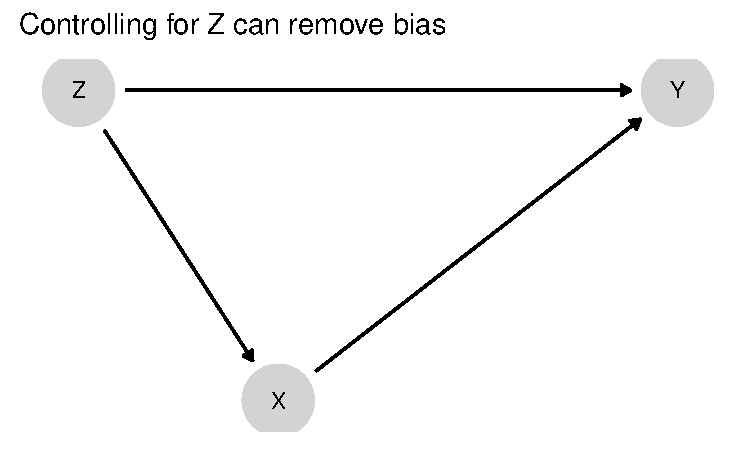
\includegraphics{2.2_estimands_files/figure-beamer/unnamed-chunk-11-1.pdf}

}

\end{figure}
\end{frame}

\begin{frame}{Confounding}
\protect\hypertarget{confounding}{}
Example where \(Z\) is correlated with \(X\) and \(Y\) but it is
\emph{not} a confounder

\begin{figure}

{\centering 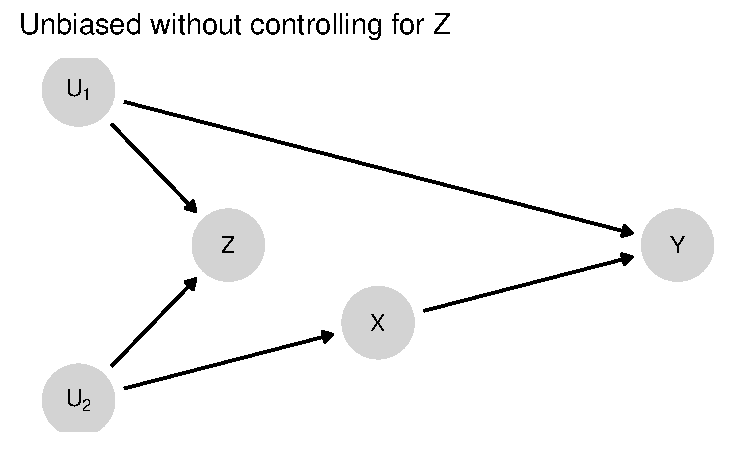
\includegraphics{2.2_estimands_files/figure-beamer/unnamed-chunk-12-1.pdf}

}

\end{figure}
\end{frame}

\begin{frame}{Important Examples : Collider}
\protect\hypertarget{important-examples-collider}{}
But controlling can also cause problems. In fact conditioning on a
temporally pre-treatment variable could cause problems. Who'd have
thunk? Here is an example from Pearl (2005):

\begin{figure}

{\centering 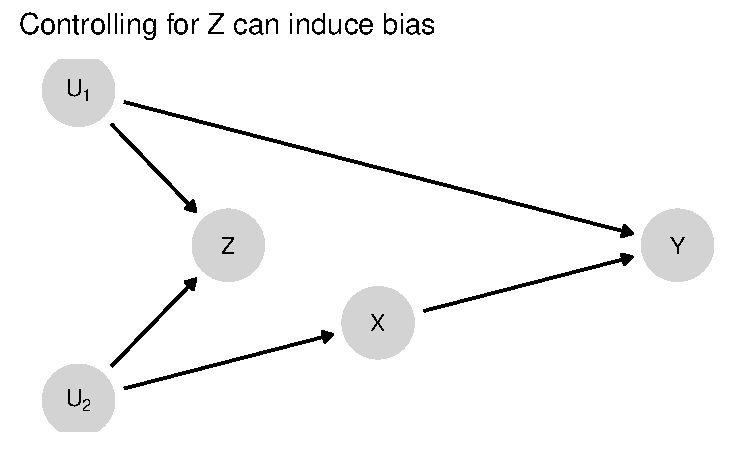
\includegraphics{2.2_estimands_files/figure-beamer/unnamed-chunk-13-1.pdf}

}

\end{figure}
\end{frame}

\begin{frame}[fragile]{Illustration of identification failure from
conditioning on a collider}
\protect\hypertarget{illustration-of-identification-failure-from-conditioning-on-a-collider}{}
\begin{Shaded}
\begin{Highlighting}[]
\NormalTok{U1 }\OtherTok{\textless{}{-}} \FunctionTok{rnorm}\NormalTok{(}\DecValTok{10000}\NormalTok{);  U2 }\OtherTok{\textless{}{-}} \FunctionTok{rnorm}\NormalTok{(}\DecValTok{10000}\NormalTok{)}
\NormalTok{Z  }\OtherTok{\textless{}{-}}\NormalTok{ U1}\SpecialCharTok{+}\NormalTok{U2}
\NormalTok{X  }\OtherTok{\textless{}{-}}\NormalTok{ U2 }\SpecialCharTok{+} \FunctionTok{rnorm}\NormalTok{(}\DecValTok{10000}\NormalTok{)}\SpecialCharTok{/}\DecValTok{2}
\NormalTok{Y  }\OtherTok{\textless{}{-}}\NormalTok{ U1}\SpecialCharTok{*}\DecValTok{2} \SpecialCharTok{+}\NormalTok{ X}

\FunctionTok{lm\_robust}\NormalTok{(Y }\SpecialCharTok{\textasciitilde{}}\NormalTok{ X) }\SpecialCharTok{|\textgreater{}} \FunctionTok{tidy}\NormalTok{() }\SpecialCharTok{|\textgreater{}} \FunctionTok{kable}\NormalTok{(}\AttributeTok{digits =} \DecValTok{2}\NormalTok{)}
\end{Highlighting}
\end{Shaded}

\begin{tabular}{l|r|r|r|r|r|r|r|l}
\hline
term & estimate & std.error & statistic & p.value & conf.low & conf.high & df & outcome\\
\hline
(Intercept) & -0.02 & 0.02 & -0.85 & 0.39 & -0.06 & 0.02 & 9998 & Y\\
\hline
X & 0.98 & 0.02 & 54.27 & 0.00 & 0.94 & 1.02 & 9998 & Y\\
\hline
\end{tabular}

\begin{Shaded}
\begin{Highlighting}[]
\FunctionTok{lm\_robust}\NormalTok{(Y }\SpecialCharTok{\textasciitilde{}}\NormalTok{ X }\SpecialCharTok{+}\NormalTok{ Z) }\SpecialCharTok{|\textgreater{}} \FunctionTok{tidy}\NormalTok{() }\SpecialCharTok{|\textgreater{}} \FunctionTok{kable}\NormalTok{(}\AttributeTok{digits =} \DecValTok{2}\NormalTok{)}
\end{Highlighting}
\end{Shaded}

\begin{tabular}{l|r|r|r|r|r|r|r|l}
\hline
term & estimate & std.error & statistic & p.value & conf.low & conf.high & df & outcome\\
\hline
(Intercept) & -0.01 & 0.01 & -0.65 & 0.51 & -0.02 & 0.01 & 9997 & Y\\
\hline
X & -0.33 & 0.01 & -35.01 & 0.00 & -0.35 & -0.31 & 9997 & Y\\
\hline
Z & 1.67 & 0.01 & 225.73 & 0.00 & 1.65 & 1.68 & 9997 & Y\\
\hline
\end{tabular}
\end{frame}

\begin{frame}[fragile]{Let's look at that in dagitty}
\protect\hypertarget{lets-look-at-that-in-dagitty}{}
\begin{Shaded}
\begin{Highlighting}[]
\NormalTok{g }\OtherTok{\textless{}{-}} \FunctionTok{dagitty}\NormalTok{(}\StringTok{"dag\{U1 {-}\textgreater{} Z  ; U1 {-}\textgreater{} y ; U2 {-}\textgreater{} Z ; U2 {-}\textgreater{} x  {-}\textgreater{} y\}"}\NormalTok{)}
\FunctionTok{adjustmentSets}\NormalTok{(g, }\AttributeTok{exposure =} \StringTok{"x"}\NormalTok{, }\AttributeTok{outcome =} \StringTok{"y"}\NormalTok{)}
\end{Highlighting}
\end{Shaded}

\{\}

\begin{Shaded}
\begin{Highlighting}[]
\FunctionTok{isAdjustmentSet}\NormalTok{(g, }\StringTok{"Z"}\NormalTok{, }\AttributeTok{exposure =} \StringTok{"x"}\NormalTok{, }\AttributeTok{outcome =} \StringTok{"y"}\NormalTok{)}
\end{Highlighting}
\end{Shaded}

{[}1{]} FALSE

\begin{Shaded}
\begin{Highlighting}[]
\FunctionTok{isAdjustmentSet}\NormalTok{(g, }\ConstantTok{NULL}\NormalTok{, }\AttributeTok{exposure =} \StringTok{"x"}\NormalTok{, }\AttributeTok{outcome =} \StringTok{"y"}\NormalTok{)}
\end{Highlighting}
\end{Shaded}

{[}1{]} TRUE

Which means, no need to condition on anything.
\end{frame}

\begin{frame}{Collider \& Confounder}
\protect\hypertarget{collider-confounder}{}
A bind: from Pearl 1995.

\begin{figure}

{\centering 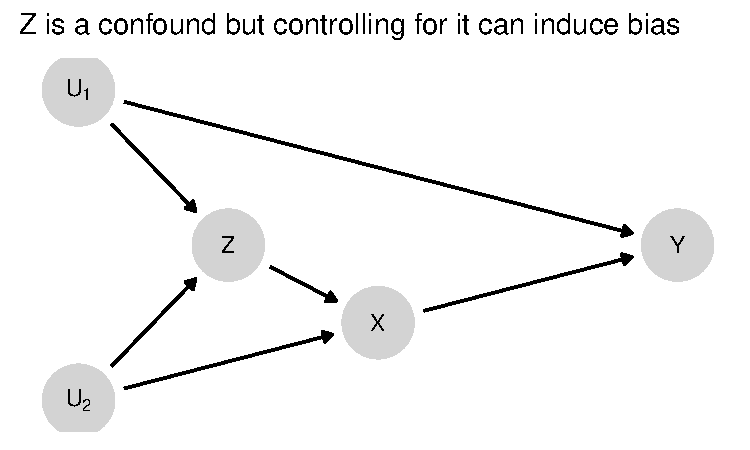
\includegraphics{2.2_estimands_files/figure-beamer/unnamed-chunk-16-1.pdf}

}

\end{figure}

For a solution for a class of related problems see @robins2000marginal
\end{frame}

\begin{frame}[fragile]{Let's look at that in dagitty}
\protect\hypertarget{lets-look-at-that-in-dagitty-1}{}
\begin{Shaded}
\begin{Highlighting}[]
\NormalTok{g }\OtherTok{\textless{}{-}} \FunctionTok{dagitty}\NormalTok{(}\StringTok{"dag\{U1 {-}\textgreater{} Z  ; U1 {-}\textgreater{} y ; }
\StringTok{             U2 {-}\textgreater{} Z ; U2 {-}\textgreater{} x  {-}\textgreater{} y; }
\StringTok{             Z {-}\textgreater{} x\}"}\NormalTok{)}
\FunctionTok{adjustmentSets}\NormalTok{(g, }\AttributeTok{exposure =} \StringTok{"x"}\NormalTok{, }\AttributeTok{outcome =} \StringTok{"y"}\NormalTok{)}
\end{Highlighting}
\end{Shaded}

\{ U1 \} \{ U2, Z \}

which means you have to adjust on an unobservable. Here we double check
that including or not including ``Z'' is enough:

\begin{Shaded}
\begin{Highlighting}[]
\FunctionTok{isAdjustmentSet}\NormalTok{(g, }\StringTok{"Z"}\NormalTok{, }\AttributeTok{exposure =} \StringTok{"x"}\NormalTok{, }\AttributeTok{outcome =} \StringTok{"y"}\NormalTok{)}
\end{Highlighting}
\end{Shaded}

{[}1{]} FALSE

\begin{Shaded}
\begin{Highlighting}[]
\FunctionTok{isAdjustmentSet}\NormalTok{(g, }\ConstantTok{NULL}\NormalTok{, }\AttributeTok{exposure =} \StringTok{"x"}\NormalTok{, }\AttributeTok{outcome =} \StringTok{"y"}\NormalTok{)}
\end{Highlighting}
\end{Shaded}

{[}1{]} FALSE
\end{frame}



\end{document}
